%!TEX root = ../thesis.tex

\cleardoublepage
\chapter{Evaluation}
\label{cha:evaluation}

This chapter looks at the set-up for the experiments and the results achieved. First, in section \ref{sec:testing} the environment in which the agents were tested is explained and then in the section \ref{sec:analysis} the results are presented and discussed. 

\textbf{TODO: move this to conclusion section} Then section \ref{sec:_pot_improvements} considers what could be improved or done differently . Finally section \ref{sec:implications} looks forwards and asks what implications this could have and what the next steps would be.


\section{Testing the Agents}
\label{sec:testing}

In order to evaluate the performance of these agents they were tested on a 32-core, 125GB RAM machine against 5 different workflows from the popular bioinformatics framework nf-core \footnote{https://nf-co.re/}. Each workflow is run 10 times without any reinforcement learning agents active. This was done to have something to compare the results to later but also so that there was historical data about the average time each of the tasks take since the reinforcement learning agents need this information. After that the agents are tested. The gradient bandits are run 50 times for each workflow and the q-learning agents 100 times. As has been explained in \ref{subsub:states} the q-learning agent needs considerably longer to explore its extensive state-action space and as such is run for longer. However even though it is run twice as many times, the q-learning agent is still perhaps under-trained since the state-action space it needs to explore is so much larger than the action-space which the gradient bandits explore. 

Four different reinforcement learning agents are trained: the CPU bandit, a co-location of the CPU bandit and the memory bandit, the CPU only q-learning agent, and the CPU and memory q-learning approach. 

The five workflows used are the following: 1) \textit{eager} - a pipeline for genomic NGS sequencing data, 2) \textit{mhcquant} - a workflow for quantitative processing of data dependent (DDA) peptidomics data, 3) \textit{nanoseq} - which is an analysis pipeline for Nanopore DNA/RNA sequencing data, 4) \textit{viralrecon}- which can be  used to perform assembly and intra-host/low-frequency variant calling for viral sample, and 5)  \textit{metaboigniter} - a pipeline for pre-processing of mass spectrometry-based metabolomics data. 

The input data used for the workflows is based on custom combinations of different input files provided by the workflow's maintainers. Generally for each pipeline there are full example datasets and short example datasets as well as configurations for each of them. The short datasets are all configured to only assign either 1 or 2 CPUs and are thus are not really feasible for comparison, however the full datasets, whilst featuring realistic configurations, often take far too long to run. For reference, the full datasets will often take 6 hours or more to run once whereas the short examples never take more than 5 minutes. In order to build good pipelines with more realistic runtimes, configurations and input data, but without running too long, the short examples and the full ones need to be combined. The combinations are designed to strike a balance between having large input data and realistic task configurations but also being short enough that it is feasible to run the workflows hundreds of times. Each one is built differently but the overarching tactic used was to start with the command line arguments to the pipeline from the short examples and combine it with the configuration and the input data from the full dataset. After this the list of input files is reduced until the pipeline completes in a reasonable amount of time. Ultimately, by following this process, configurations and inputs were found for all five of the pipelines mentioned above such that they were completing after around 10 to 40 minutes.  

The nextflow source code inherently keeps track of the total number of resources available and the resources already assigned to tasks and it will not schedule more resources than the system has. The tasks are all run inside of docker containers with the exact amount of CPUs and memory requested by the task. Since the tasks are all being run on the same machine it would have been possible to ignore the sum of the resource requests and over-assign resources so that all of the tasks compete with each other, but this does not reflect situations where pipelines are being run on clusters with resource managers, and as such this was left unchanged.

For the final comparison in the evaluation chapter the 10 runs with the default configurations are compared to the last 10 runs with each of the agents.



%%=========================================
\section{Analysis of Results}
\label{sec:analysis}

\subsection{Performance Comparison}
\label{sub:comp_perf}

\begin{figure}
    \centering
        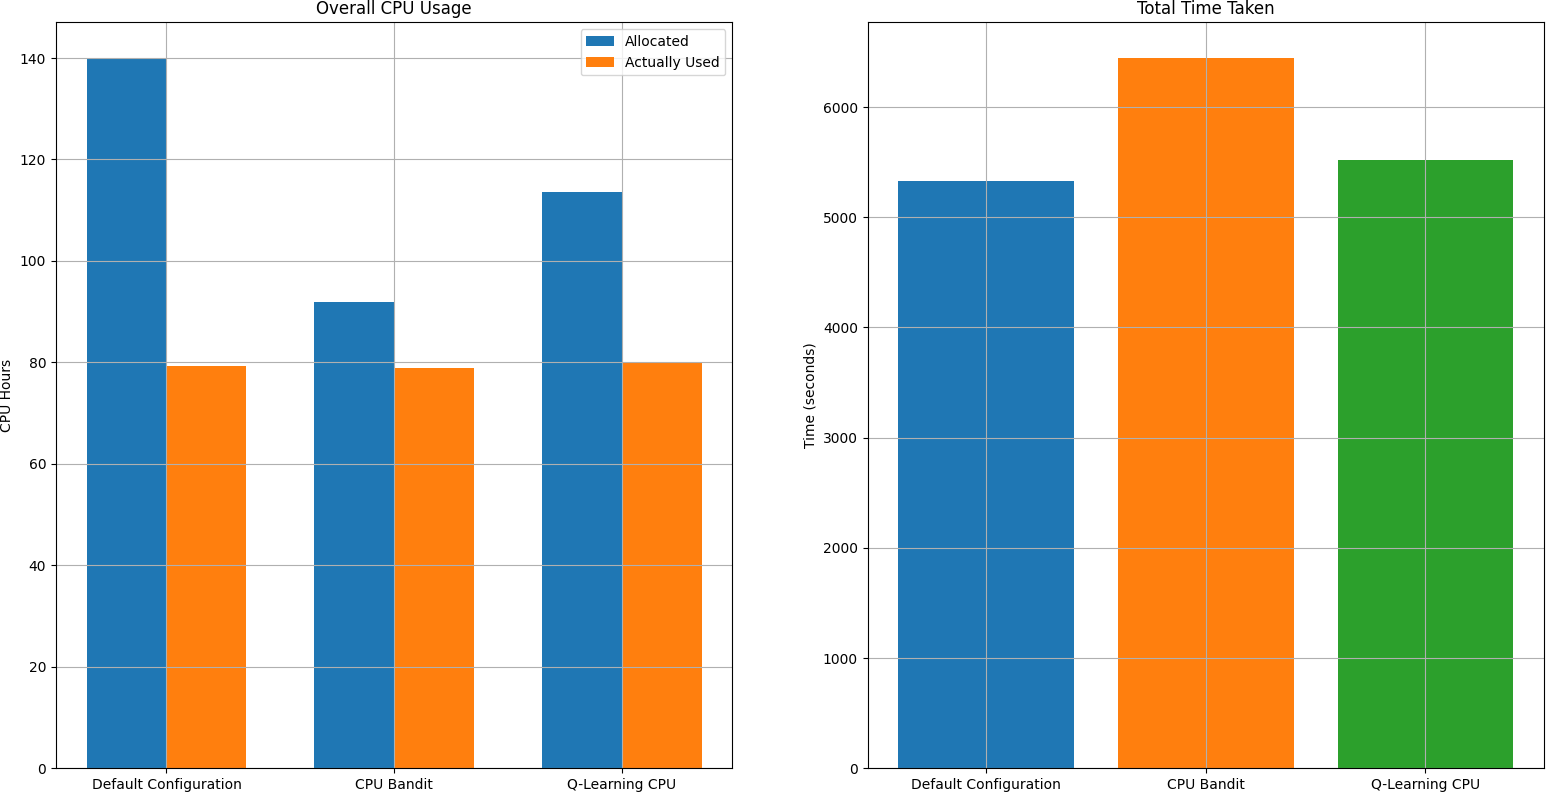
\includegraphics[width=\textwidth]{fig/cpu_only_results.png}
        \caption{Comparison of workflow performance for the approaches which only change CPU}
        \label{fig:cpu_results}
\end{figure}

\begin{figure}
    \centering
        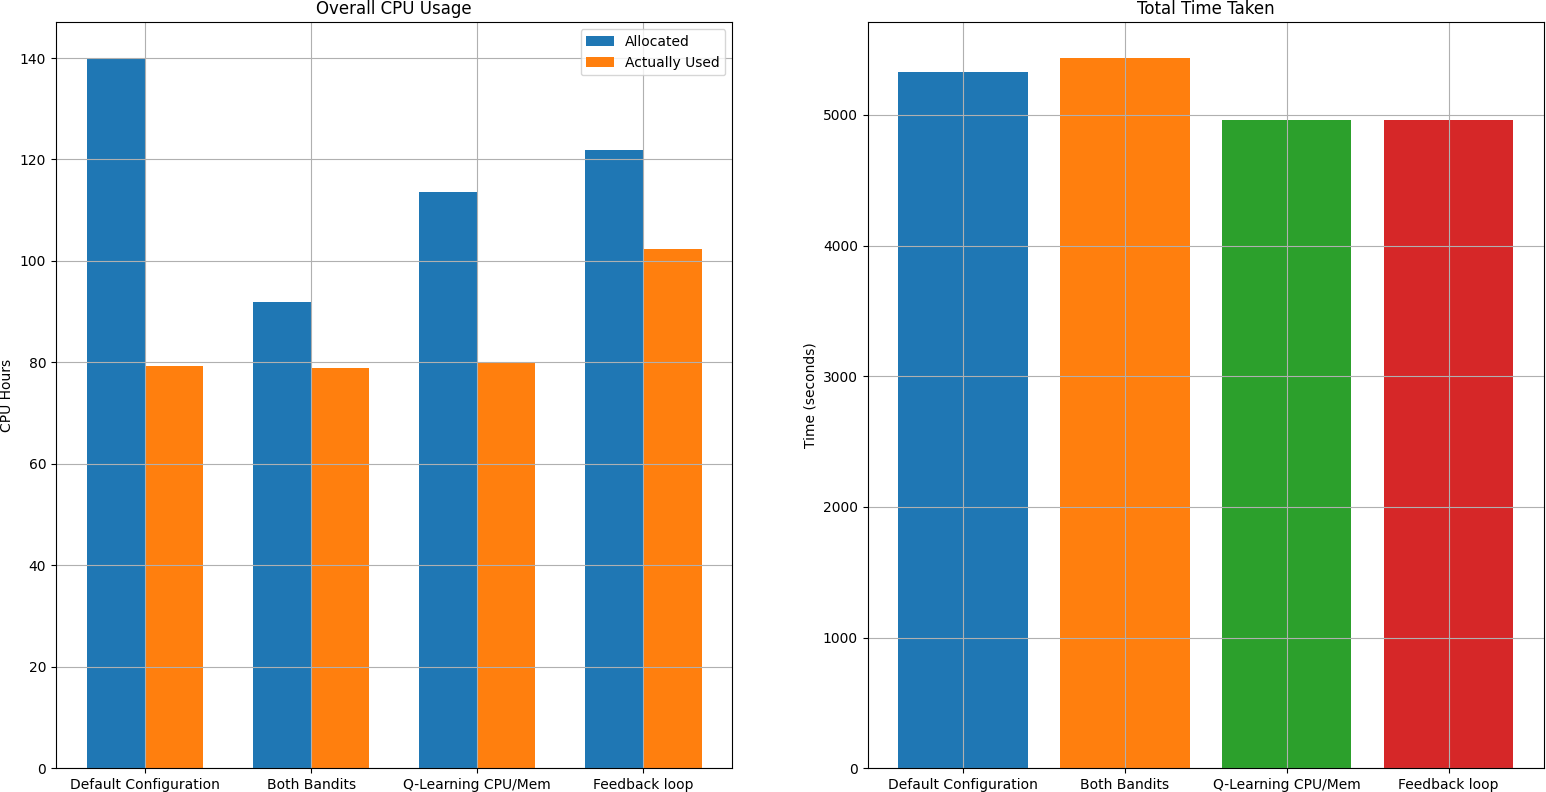
\includegraphics[width=\textwidth]{fig/cpu_mem_results.png}
        \caption{Comparison of workflow performance for the approaches which change CPU and Memory}
        \label{fig:mem_results}
\end{figure}

\begin{figure}
    \centering
        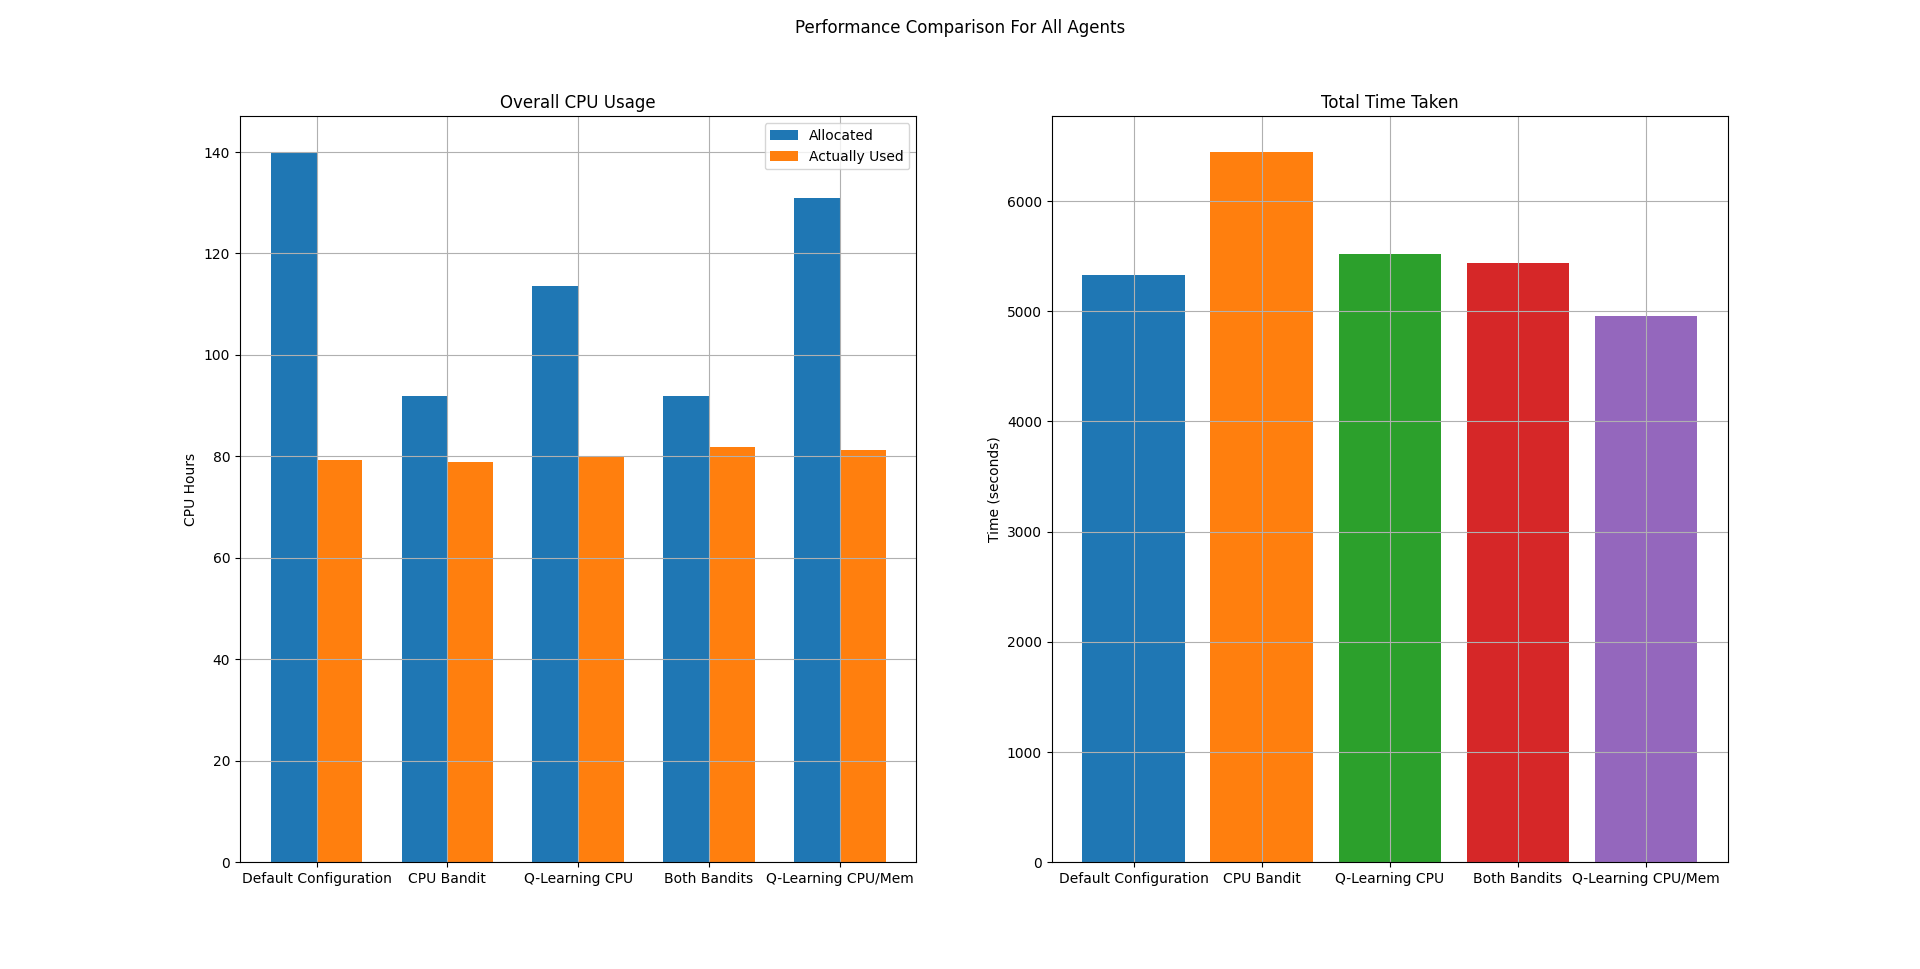
\includegraphics[width=\textwidth]{fig/all_results.png}
        \caption{Performance comparison of all of the approaches}
        \label{fig:all_results}
\end{figure}

\begin{figure}
    \centering
        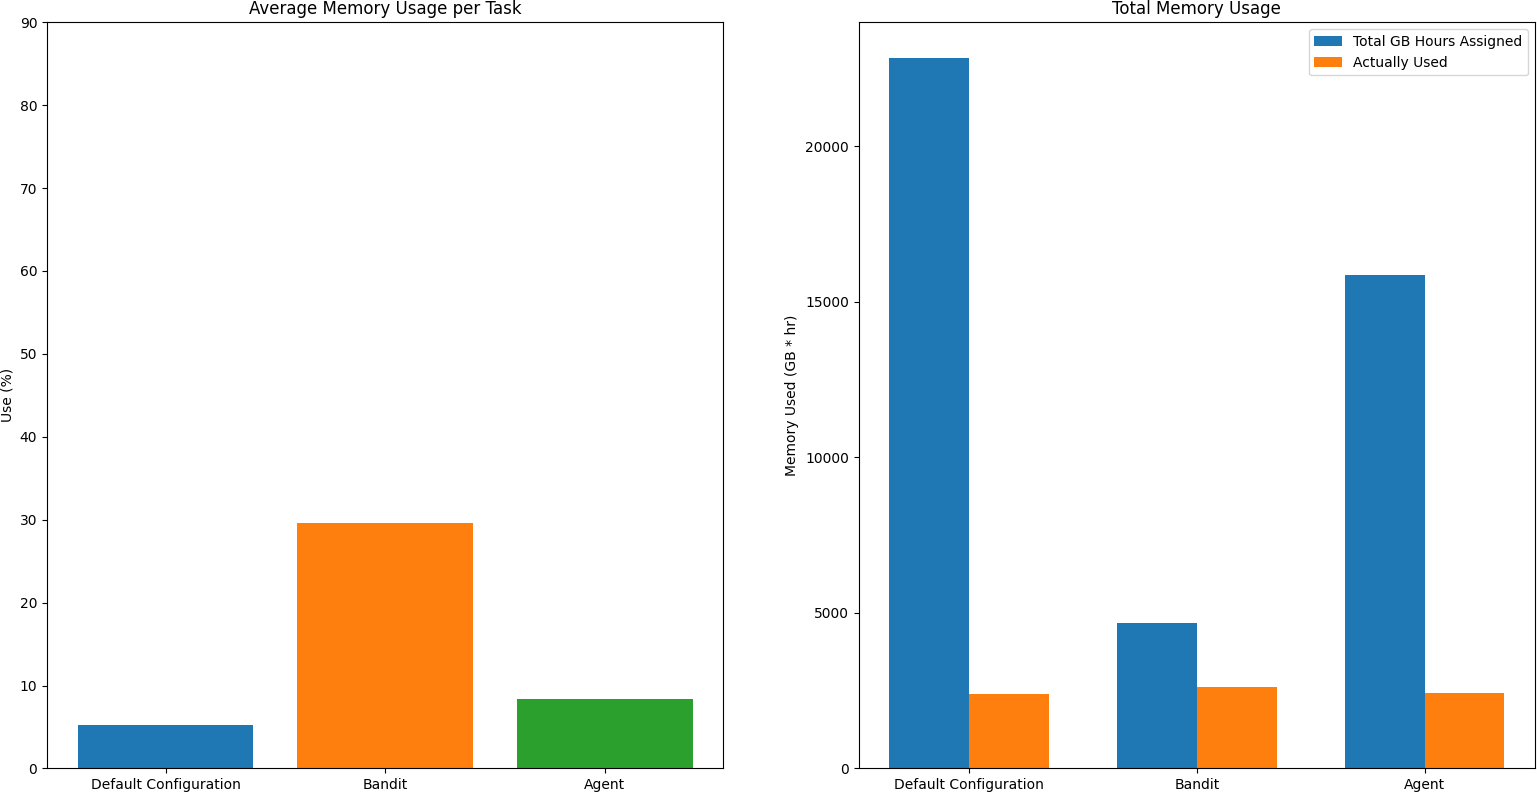
\includegraphics[width=\textwidth]{fig/cropped_memory_usage_final.png}
        \caption{Memory Usage}
        \label{fig:mem_use}
\end{figure}

In this section the performance of the gradient bandit and the q-learning approaches over their last 10 runs will be compared with each other and with the performance of 10 runs of the same workflows with their default configuration.

The figures \ref{fig:cpu_results}, \ref{mem_results} and \ref{fig:all_results} show the performance of the different approaches and compare them to the default configuration. The left graph looks at the total amount of CPU hours requested across all of the workflows and the amount of CPU hours that were actually used. The right graph in these 3 figures shows the total time it took for all of the workflows to complete. Finally in \ref{fig:mem_use}, the memory usage is shown. The unit measured is the gigabyte hour and the graphic displays the total amount of gigabyte hours allocated across all of the runs as well as the actual amount of gigabyte hours used (based on the task’s peak RSS and execution time). Since the CPU bandit and the CPU only q-learning approach did not alter memory they are not shown.

From these graphics it is clear to see that all of the reinforcement learning approaches managed to improve CPU efficiency and allocate less CPU Hours than the default configuration. In the case of the gradient bandits they were both particularly effective at keeping the overall CPU hours assigned to an absolute minimum, however it seems that this efficiency came at the cost of speed and they both performed worse than their q-learning counterparts in this aspect. The q-learning approach for both memory and CPUs was the least efficient (ignoring the default configurations). However this approach was still more efficient than the default configurations and the only approach which was faster than the default configuration. Indeed these figures make it clear that assigning less CPU hours generally seems to have a detrimental effect on runtime (as may be expected) but the change in efficiency is much greater than the change in runtime. Thus it should not be particularly surprising that the fastest agent assigned the most resources of any reinforcement learning approach. 

With regards to memory both of the reinforcement learning approaches proved to be significantly better than the default configuration with regards to this resource. One aspect which stands out is firstly how poor the default configurations are. Indeed they are just about using 10\% of the assigned memory and performing even worse on a task by task basis . On the other hand the q-learning approach is not much more efficient however it still reduces the overall amount of wasted memory by a large amount. The best performer by a significant margin is the memory bandit and this approach yields much better results. In fact it assigns less than half as much as either the default configuration or the q-learning agent. 

A noticeable trend is that both of the approaches which also reduce memory are able to achieve much better total runtimes than the other two approaches which only alter CPU. This is clearly down to the large overestimations for memory use contained in the default configuration. Since nextflow only executes tasks whose resource requirements can be fulfilled by the unassigned resources which remain available to the execution platform, the excessive memory requests from the tasks in the default configuration were most likely preventing other tasks from executing and by re-sizing these requests, the two memory altering approaches were able to achieve greater task throughput and reduced runtimes. In closing it should also be pointed out the both of the q-learning approaches were faster but less efficient with CPU hours than their gradient bandit counterparts and this may be down to the different reward functions used, since the q-learning approaches set a cap on the CPU usage’s influence on the reward function. Looking at the reward functions \ref{q_agent_1_reward} and \ref{q_agent_2_reward} the CPU usage which is used in the function is not the usage of the task but rather $max(90,CPU\_usage)$. As such agent’s for tasks which exhibit very high CPU usage ($>90\%$) receive no additional reward for increased efficiency (since efficiency can always be increased by decreasing the total number of CPUs assigned) so their rewards depend entirely on the execution time and they are thus encouraged to assign more resources and try to decrease runtime.

\subsection{Summary of Results}
\label{sub:summary}

In conclusion all of the reinforcement learning approaches were able to intelligently size the tasks in the workflows and in the end the overall number of CPU hours which were wasted was reduced. In addition to this the agents were also able to significantly reduce the memory usage. The gradient bandits took slightly longer on average but were much more efficient for that, whilst the q-learning agents struck a better balance between resource efficiency and increased performance and the q-learning approach for both CPU and memory was ultimately able to outperform the default configurations in both efficiency and runtime.

While it could be argued that the q-learning agents are therefore the “better” options it is hard to say exactly what the right approach is because it also depends on the desires of the user. Many scientists may be prepared to accept slightly longer runtimes if the “greediness” of their workflows is decreased and they are able to free up resources for others to use, or reduce their own costs (if they are paying for CPU hours). Indeed from a financial perspective the gradient bandit wastes significantly less CPU hours than the extra time it takes to complete. However in a situation where the user is paying for the entire system (and not resource usage) it may make more sense from a financial perspective to use the q-learning agent approach since it reduces the amount of time for which the system needs to be up.
